\documentclass[11pt,a4paper]{article}
\usepackage[latin1]{inputenc}
\usepackage{amsmath}
\usepackage{amsfonts}
\usepackage{amssymb}
\usepackage{graphicx}
\author{Jordan Murray}
\title{EECS305 Lab5}
\begin{document}
\begin{center}
\fontsize{24}{12}\selectfont
\textbf{Experiment 5: Lead-Lag Control of a DC Servo Motor}
\end{center}
\section{OBJECTIVES}

\begin{enumerate}
\item Frequency domain

\item bode plot

\item phase margin

\end{enumerate}


\section{BASIC KNOWLEDGE}
In this experiment, we introduce mathematical models for a DC servomechanism and lead-lag compensator design using the root-locus method

\subsection{Background information on DC servo motor system}

A block diagram for a typical servomechanism is shown in Fig. ~\ref{fig:servoblock}.  The action of the servomechanism is to track a desired position (or speed) despite the 
presence of disturbance inputs to the process and despite errors in the 
sensor data.

\begin{figure}[here]
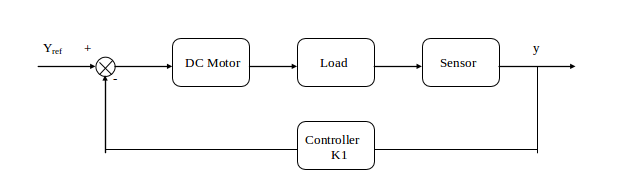
\includegraphics[width=\textwidth]{imglab/servoblockdiagram.png}
\caption{Servomechanism block diagram}
\label{fig:servoblock}
\end{figure}

\subsubsection{Model Development}
\begin{figure}[here]
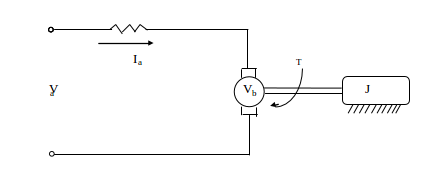
\includegraphics[width=\textwidth]{imglab/servoschemdiagram.png}
\caption{schematic diagram of the DC servo motor}
\label{fig:servoschem}
\end{figure}

We begin by developing a simplified linear model of an armature controlled DC servo motor and load. Fig. ~\ref{fig:servoschem} shows the schematic diagram of the motor and load.

Neglecting the inductance of the armature circuit, the armature voltage V$_{a}$ produces a current I$_{a}$ as given by:

\begin{equation} \label{eq:1}
I_{a} = \frac{V_{a}-V_{b}}{R_{a}}
\end{equation}

Here V$_{b}$ denotes the back emf of the motor and R$_{a}$ is the armature resistance.

The motor torque T is proportional to I$_{a}$:

\begin{equation} \label{eq:2}
T = K_{T}I_{a}
\end{equation}

But from Newton's law, assuming an inertia load:

\begin{equation} \label{eq:3}
T = J\ddot{\theta}
\end{equation}

combining equations \ref{eq:1}, \ref{eq:2}, and \ref{eq:3} we obtain:

\begin{equation} \label{eq:4}
K_{T}\left[\frac{V_{a}-V_{b}}{R_{a}}\right] = J\ddot{\theta}
\end{equation} 

Using the relationship V$_{b}$ = K$_{b}\dot{\theta}$ and, letting V$_{a}$ = U (input signal), we have:

\begin{equation} \label{eq:5}
\frac{K_{T}}{R_{a}}\left[U-K_{b}\dot{\theta}\right] = J\ddot{\theta}
\end{equation}

\begin{equation} \label{eq:6}
\frac{JR_{a}}{K_{T}}\ddot{\theta}+ K_{b}\dot{\theta} = U
\end{equation}

\begin{equation} \label{eq:7}
\ddot{\theta} + \frac{K_{b}K_{T}}{JR_{a}}\dot{\theta} = \frac{K_{T}}{JR_{a}}U
\end{equation}

or letting $\omega$ = $\dot{\theta}$, and 

\begin{equation} \label{eq:8}
\dot{\omega} + \frac{K_{b}K_{T}}{JR_{a}}\omega = \frac{K_{T}}{JR_{a}}U
\end{equation}

Equations \ref{eq:7} and \ref{eq:8} are the differential equations for the DC motor.

Let $\frac{K_{b}K_{T}}{JR_{a}} = \frac{1}{\tau}$, $\frac{K_{T}}{JR_{a}} = \frac{K_{0s}}{\tau}$. Here, $K_{0s}$ is the static gain and $\tau$ is the time constant of the system from input voltage to output speed. From D.E. \ref{eq:7} we can have the following transfer function:

\begin{equation} \label{eq:9}
\frac{\theta(s)}{U(s)} = \frac{K_{0s}}{s(\tau s + 1)}
\end{equation}

And from D.E. \ref{eq:8} we obtain the transfer function of the DC motor from U to $\dot{\theta}=\omega$:

\begin{equation} \label{eq:10}
\frac{\omega (s)}{U(s)} = \frac{K_{0s}}{(\tau s + 1)}
\end{equation}

Considering the measurements of speed and position, the system can be depicted as in Fig. ~\ref{fig:servomeasschem}

\begin{figure}[here]
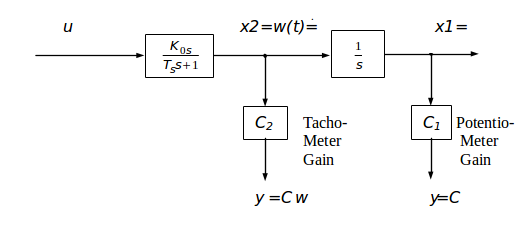
\includegraphics[width=\textwidth]{imglab/servomeasurementschematic.png}
\caption{schematic of the DC motor system with measurements}
\label{fig:servomeasschem}
\end{figure}

Then, the second order D.E. of the DC motor can be rewritten in the state-space format:

$x = A\dot{x} + Bu$
$y = Cx$

where, $x = \left[\begin{matrix}x_{1} \\ x_{2}\end{matrix}\right]$, $u=u$, $y = \left[\begin{matrix}y_{1} \\ y_{2}\end{matrix}\right]$, and
$A = \left[\begin{matrix}0 & 1 \\ 0 & -\frac{1}{\tau}\end{matrix}\right]$, $B=\left[\begin{matrix} 0 \\ \frac{K_{s}}{\tau} \end{matrix}\right]$, $C = \left[\begin{matrix}C_{1} & 0 \\ 0 & C_{2} \end{matrix}\right]$

Further, the input/output transfer function of the DC motor is:

\begin{equation} \label{eq:11}
G(s)=\frac{Y(s)}{U(s)} = \left[ \begin{matrix} G_{1}(s) \\ G_{2}(s) \end{matrix} \right] = \left[ \begin{matrix} \frac{C_{1}K_{0x}}{s(\tau s + 1)} \\ \frac{C_{2}K_{0s}}{\tau s + 1} \end{matrix} \right] = \left[ \begin{matrix} \frac{\left(\frac{C_{1}}{C_{2}}\right)*C_{2}K_{0s}}{s(\tau s + 1)} \\ \frac{C_{2}K_{0s}}{\tau s + 1} \end{matrix} \right]
\end{equation}

Define: $C_{s}=C_{1}/C_{2} and K_{s}=C_{2}K_{0s}$, then

\begin{equation} \label{eq:12}
G(s)=\frac{Y(s)}{U(s)} = \left[ \begin{matrix} G_{1}(s) \\ G_{2}(s) \end{matrix} \right] = \left[ \begin{matrix} \frac{C_{s}K_{s}}{s(\tau s + 1)} \\ \frac{K_{s}}{\tau s + 1} \end{matrix} \right]
\end{equation}

The model has one pole at the origin and one pole on the negative real axis. The problem is to identify parametesr $K_{s}, \tau$ and $C_{s}$. From \ref{eq:12}, the transfer function from input u to output $y_{2}$ is:

\begin{equation} \label{eq:13}
\frac{Y_{2}(s)}{U(s)} = \frac{K_{s}}{\tau s + 1}
\end{equation}

The step response of the first order system is shown in Fig. ~\ref{fig:servostepresp}:

\begin{figure}[here]
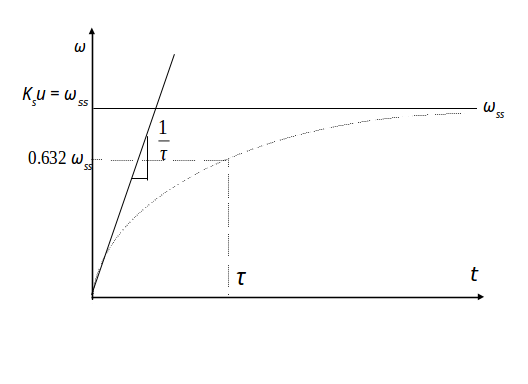
\includegraphics[width=\textwidth]{imglab/servostepresponse.png}
\caption{step response of the DC servo motor}
\label{fig:servostepresp}
\end{figure}

From this diagram, we can determine that the time constant of the motor, $\tau$, is the time it takes $y_{2}$ to reach 63.2\% of its steady state value $y_{2ss}$. We can also obtain the steady-state gain $K_{s} = \frac{y_{2ss}}{U_{ss}}$.

In addition, notice that regarding $C_{s}$ there is a conformity that has to be satisfied:

\begin{equation} \label{eq:14}
C_{s} = \frac{\frac{dy_{1}}{dt}}{y_2}
\end{equation}
This gives the way to identify $C_{s}$.

\subsubsection{Closed Loop Control for a DC servomechanism}
The block diagram of Fig. ~\ref{fig:servoblock} for the servomechanism can be simplified into the block diagram given in Fig. ~\ref{fig:servotfblock}.

\begin{figure}[here]
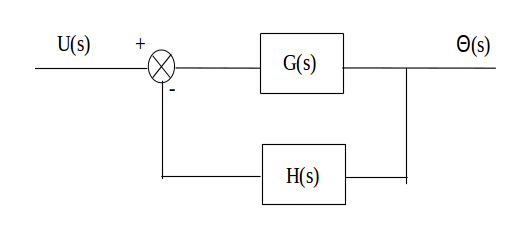
\includegraphics{imglab/servotfblock.png}
\caption{simplified block diagram}
\label{fig:servotfblock}
\end{figure}

This configuration is referred to as a negative feedback closed loop configuration where G(s) is the forward loop transfer function and H(s) is the feedback loop transfer function. The equivalent transfer function between the input r(t) and the output y(t) as shown in Fig. ~\ref{fig:servostepresp} can be represented as the transfer function G'(s) shown in Fig. ~\ref{fig:servocltfblock}.

\begin{figure}[here]
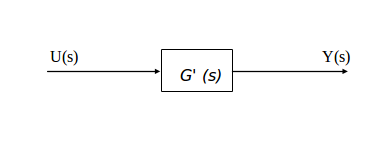
\includegraphics{imglab/servocltfblock.png}
\caption{eqivalent closed-loop transfer function}
\label{fig:servocltfblock}
\end{figure}

\begin{equation} \label{eq:15}
G'(s)=\frac{Y(s)}{U(s)}=\frac{G(s)}{1+G(s)H(s)}
\end{equation}

Considering the servomechanism transfer function:

From Eq. \ref{eq:9}: $G(s)=\frac{C_{s}K_{s}}{s(\tau s + 1)}$,

H(s) = K$_{1}$ (Output feedback controller gain),

\begin{equation} \label{eq:16}
G'(s)=\frac{\frac{C_{s}K_{s}}{\tau}}{s^{2} + \frac{s}{\tau} + \frac{K_{1}K_{s}C_{s}}{\tau}}
\end{equation}

We observe that the transfer function of the closed-loop system, G'(s) is a second order system with one free controller parameter $K_{1}$. Changing the gain $K_{1}$ can be used to alter the transient dynamics of the second order system.

\subsection{Background information on lead-lag compensator design}
Lead and lag compensators are used quite extensively in control. A lead compensator can increase the stability or speed of response of a system; a lag compensator can reduce (but not eliminate) the steady state error. If improvements in both transient response and steady-state response are desired, then both a lead compensator and a lag compensator may be used simultaneously. Depending on the effect desired, one or more lead and lag compensators may be used in various combinations.

%\subsubsection{Lead compensator}

%\subsubsection{Lag compensator}

\section{EXPERIMENTAL PROCEDURES}
\subsection{Identify $K_{s}$, $\tau$, $C_{s}$:}
\begin{enumerate}
\item You should have identified these parameters of the DC servo model in a previous lab. If you know the values of these parameters you can skip to the lead compensator design section.

\item Run \textbf{MATLAB} and open the model \textbf{Lab5\_identification.slx}. The \textit{DC servo} block contains a masked model of a DC servo motor. Run the model. A unit step input is applied to the motor winding at t = 1s. Open the scope and look at the angular velocity trace. Determine the steady-state speed of the motor. This is the value of $K_{s}$, the steady-state gain. Determine the time at which the speed reaches 63.2\% of its final value. Find the elapsed time since the step function was applied. This value is the time constant $\tau$.

\item Again using the scope, determine the slope of the asymptote of the angle trace. This is another way of measuring the angular velocity which allows us to determine $C_{s}$ (see Eq. \ref{eq:14}). 
\end{enumerate}

\subsection{Lead Compensator Design} \label{ss:specs}
\begin{enumerate}
\item From \textbf{3.1} we know system parameters $K_{s}$, $\tau$, $C_{s}$, with which we can estimate the transfer function of the motor and design a controller accordingly.

\item The transient response specifications are as follows:
\begin{enumerate}
\item Maximum percentage overshoot less than 5%
\item Settling time (2\% band) less than 1 second
\end{enumerate}

Calculate the corresponding restrictions on the values of the damping ratio $\zeta$ and the natural frequency $\omega_{n}$.


\item Determine our desired closed loop dominant pole locations from the $\zeta$ and $\omega_{n}$ calculated in the previous step. You might try selecting the points at the intersections of the constraining curves from the previous step.

\item  The open loop system consisting of the controller and plant has 1 zero and 3 poles. The open loop plant poles are fixed at zero and 1/$\tau$. The compensator pole and zero must be chosen so that the root locus intersects the desired pole location. The feedback gain associated with this point on the root locus must then be determined. \textit{You will have to show this work in your report.}

Suggested procedure:
\begin{enumerate}
\item Find the real axis projection of the desired pole location.
\item \label{step:zeropos} Place the controller zero at or to the left of this point on the real axis.
\item Determine where on the real axis the controller pole must be placed using the \textit{angle criterion}. Remember that a lead compensator has its pole to the left of its zero.
\item If no valid angle can be found, go back to step \ref{step:zeropos} and choose a different zero location.
\item Find the feedback gain. You might use the \textit{magnitude criterion} or the matlab command rlocfind(tf). 
\end{enumerate}

\item Record the zero, pole, and gain values.
\end{enumerate}

%\subsection{Lag Compensator Design}
%We want a lag compensator that will affect our transient response as little as possible, but will increase steady-state gain. As such, we want our pole and zero to very close to each other (consider the angle and magnitude criteria), but we also want the ratio of zero to pole to be large enough to achieve the desired steady-state gain. Both  of these requirements can be achieved if we place the zero and pole for the lag compensator near the origin. 

%Suggested procedure:
%\begin{enumerate}
%\item Place the zero to the right of the real projection of the lead compensated system's closed loop pole by a factor of 50-100.
%\end{enumerate}

\subsection{Study the transient response of the servo motor system with or without lead-lag compensator} \label{ss:transient}
Part 1:
\begin{enumerate}
\item Open the Simulink model \textbf{Lab5\_ConstantFeedback.slx}, which contains our servo model with fixed gain feedback. Set the gain to unity to start with.
\item Run the simulation. How long does it take for the angle of the motor to settle within about 2\% of the reference?
\item Increase the gain and improve on the performance. What is the shortest settling time you can obtain with a constant feedback that meets our overshoot requirements? You might use MATLAB's rlocus() to plot the root locus, sgrid() to get the boundary associated with our zeta constraint, and rlocfind() to get the gain associated with your desired closed loop pole locations.
\item Find the scope data output in the Matlab workspace and save it as a .mat file using the save command.
\end{enumerate}

Part 2:
\begin{enumerate}
\item Open the Simulink model \textbf{Lab5\_Lead.slx}, which contains our servo model with a lead compensator transfer function in the feedback path.
\item Modify the lead compensator transfer function to match the zero, pole, and gain values previously determined. 
\item Calculate the steady-state gain of the lead compensator and scale our reference signal accordingly. The reference we are providing in this configuration corresponds to the desired value of the compensator output, not the desired state measurement.
\item Run the simulation. Does the system trajectory meet the specifications? The servo model block includes a maximum control effort, which constrains the rise time. This could be an issue for some choices of pole location.
\item Find the scope data output in the Matlab workspace and save it as a .mat file using the save command.
\end{enumerate}

Part 3:
\begin{enumerate}
\item Open the Simulink model \textbf{Lab5\_Lag.slx}, which contains our servo model with a lag compensator transfer function in the forward path.
\item Note how long it takes to settle.
\item Find the scope data output in the Matlab workspace and save it as a .mat file.
\end{enumerate}

\subsection{Lead vs Lead-Lag compensation}
\begin{enumerate}
\item Open the Simulink model \textbf{Lab5\_LeadLag.slx}. This model is intended to demonstrate an application for a lag compensator. The steady state error in theta for the servo is zero for a step input since the theta-input transfer function is a type 1 system. However, the steady state error for a lead-compensated system is not zero for a ramp input. A lag compensator can reduce this error. 
\item Modify the lead compensator transfer function blocks to match the zero, pole, and gain values previously determined.
\item Run the simulation.
\item Confirm that the transient response of the step-input system is almost the same as before the addition of the lag compensator.
\item Look at the ramp input systems. Compare the error of the lead compensated system to that of the lead-lag compensated system.
\end{enumerate}



\section{REPORT}
\begin{enumerate}
\item Plot the transients responses from \ref{ss:transient}. Compare the results of the three situations. Comments are needed to describe the effects of the lead compensator and lag compensator and illustrate why they have those effects.
\item Show the detailed procedure of designing the lead compensator based on the root-locus approach. What parameters did you determine for the servo motor? What values did you calculate for $\zeta$ and $\omega_{n}$? What about the zero and pole locations and the gain for the lead compensator? Were you able to meet the specifications laid out in ~\ref{ss:specs}?
\item Design the lead compensator in a more simple way. Design a lead-lag compensator and show how and why it becomes a lead or lead-lag compensator.
\end{enumerate}
\textbf{Question:} We determined that the time constant of the motor, $\tau$, is the time it takes for $y_{2}$ to reach 63.2\% of its steady state value $y_{2ss}$, why?


\end{document}
